\documentclass[journal]{IEEEtran}
\usepackage[a5paper, margin=10mm, onecolumn]{geometry}
\usepackage{lmodern}

\setlength{\headheight}{1cm}
\setlength{\headsep}{0mm}

\usepackage{gvv-book}
\usepackage{gvv}
\usepackage{cite}
\usepackage{amsmath,amssymb,amsfonts,amsthm}
\usepackage{graphicx}
\graphicspath{{./figs/}}
\usepackage{xcolor}
\usepackage{txfonts}
\usepackage{enumitem}
\usepackage{mathtools}
\usepackage{hyperref}
\usepackage{tikz}
\usepackage{tkz-euclide}

\begin{document}

\bibliographystyle{IEEEtran}
\vspace{3cm}

\title{2.8.19}
\author{EE25BTECH11036 - M Chanakya Srinivas}
\maketitle

\renewcommand{\thetable}{\theenumi}
\setlength{\intextsep}{10pt}
\renewcommand\theequation{\arabic{equation}}


\title{Solution to Problem 2.8.19}
\author{}
\date{}
\maketitle



\section*{Problem}
Suppose for some non-zero vector \(\vec r\) we have
\[
\vec r \cdot \vec a = 0,\quad
\vec r \cdot \vec b = 0,\quad
\vec r \cdot \vec c = 0.
\]
Show that the scalar triple product \((\vec a\ \vec b\ \vec c) = 0\).

\section*{Solution}

\subsection*{Step 1: Write as matrix equation}

The three scalar equations can be written as
\begin{align}
\vec r^\top \vec a &= 0 \\
\vec r^\top \vec b &= 0 \\
\vec r^\top \vec c &= 0
\end{align}

Stack them into a single matrix equation:
\begin{align}
\myvec{
\vec a^\top \\[2mm]
\vec b^\top \\[2mm]
\vec c^\top
} \vec r
=
\myvec{0\\0\\0}.
\end{align}

\subsection*{Step 2: Define the matrix}

Let 
\begin{align}
A = \big[\vec a\ \vec b\ \vec c\big]
\end{align}
be the \(3\times 3\) matrix with columns \(\vec a,\vec b,\vec c\).  
Then the stacked equation becomes
\begin{align}
A^\top \vec r = \myvec{0\\0\\0}.
\end{align}

\subsection*{Step 3: Deduce singularity}

Since \(\vec r \neq \vec 0\) and \(A^\top \vec r = 0\), the matrix \(A^\top\) is singular. Therefore,
\begin{align}
\det(A^\top) = 0.
\end{align}

\subsection*{Step 4: Relate to scalar triple product}

But \(\det(A^\top) = \det(A)\), and the determinant of \(A\) is exactly the scalar triple product:
\begin{align}
(\vec a\ \vec b\ \vec c) = \det\big[\vec a\ \vec b\ \vec c\big] = \det(A) = 0.
\end{align}

\subsection*{Conclusion}

\[
\boxed{(\vec a\ \vec b\ \vec c) = 0}.
\]


\begin{figure}[h]
    \centering
    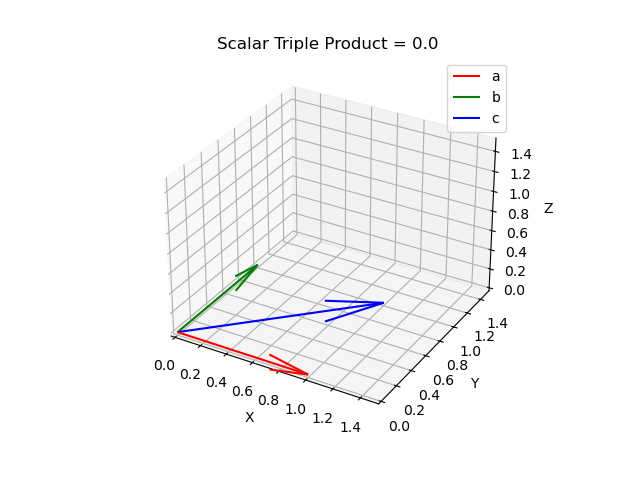
\includegraphics[width=0.9\columnwidth]{figs/fig41.png}
    \caption{}
    \label{fig:placeholder}
\end{figure}



\begin{figure}
    \centering
    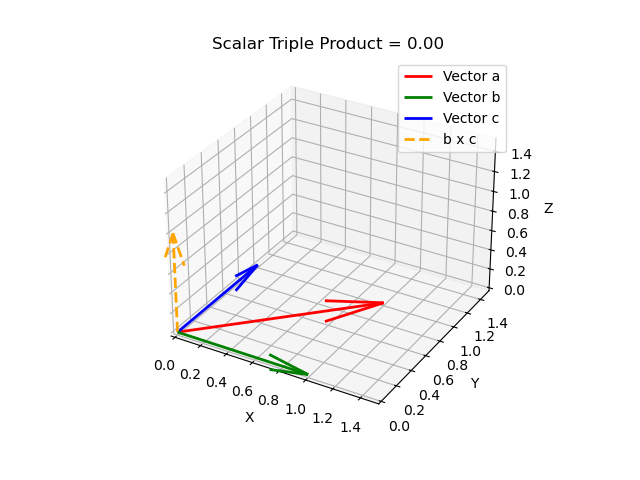
\includegraphics[width=0.9\columnwidth]{figs/fig42.png}
    \caption{}
    \label{fig:placeholder}
\end{figure}
\end{document}